
\usetikzlibrary{calc}
\usetikzlibrary {shapes.geometric}
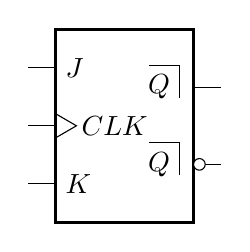
\begin{tikzpicture}[scale=0.7]
  \def\w{2.5}
  \def\h{3.5}
  \draw[line width=1.2] (0, 0) rectangle (\w, \h);
  \draw ($(0, 0)!0.8!(0,\h)$) coordinate (j) -- ++(left:0.5);
  \draw ($(0, 0)!0.5!(0,\h)$) coordinate (clk) -- ++(left:0.5);
  \draw ($(0, 0)!0.2!(0,\h)$) coordinate (k) -- ++(left:0.5);
  \draw ($(\w, 0)!0.7!(\w,\h)$) coordinate (q) -- ++(right:0.5);
  \draw ($(\w, 0)!0.3!(\w,\h)$) coordinate (nq) -- ++(right:0.5);
  
  \node[name=edge,isosceles triangle, draw, yscale=0.7, xscale=0.5, right] at (clk) {};
  
  \node[right] at (j) {$J$};
  \node[right] at (k) {$K$};
  \node[right, xshift=4] at (edge) {$CLK$};
  \node[left,name=lq, xshift=-5]  at (q) {$Q$};
  \node[left,name=lnq, xshift=-5] at (nq) {$Q$};

  \draw[fill=white,draw=black] ($(nq)+(3pt,0)$) circle (3pt);
  \draw[shorten >= 4pt, shorten <= 4pt] (lq.north west) -| (lq.south east);
  \draw[shorten >= 4pt, shorten <= 4pt] (lnq.north west) -| (lnq.south east);
  
  % Low-level effective
  % \draw[fill=white,draw=black] ($(clk)-(3pt,0)$) circle (3pt);

  % Preset and Reset signal
  % \draw (\w/2, \h) coordinate (pre) -- ++(up:0.5);
  % \draw (\w/2, 0) coordinate (cls) -- ++(down:0.5);
  % \node[below] at (pre) {$PRE$};
  % \node[above] at (cls) {$CLS$};
  % \draw[fill=white,draw=black] ($(pre)+(0,3pt)$) circle (3pt);
  % \draw[fill=white,draw=black] ($(cls)-(0,3pt)$) circle (3pt);

\end{tikzpicture}
